% !TEX encoding = UTF-8 Unicode

\documentclass[12pt,a4j,titlepage]{ltjsarticle}
\usepackage{semi}
\usepackage{here}

% \title{}
% \author{}
% \date{}

\begin{document}

\begin{titlepage}
  \begin{center}
  
    \vspace*{20truept}
    
    {\LARGE 2022年度 卒業論文}
    
    \vspace*{75truept}
    
    {\Huge 初学者向けネットワーク通信の学習を} %論文タイトル

    \vspace{10truept}

    {\Huge 支援するシミュレータWeb教材 } %論文タイトル 長い場合 改行1

    \vspace{10truept}

    {\Huge } %論文タイトル 改行2

    \vspace{85truept}
    
    {\LARGE 指導教員 須田 宇宙 准教授}
    
    \vspace{60truept}
    
    {\LARGE 千葉工業大学 情報ネットワーク学科}
    
    \vspace{15truept}
    
    {\LARGE 須田研究室}
    
    \vspace{70truept}
    
    {\LARGE 1932047 氏名 小松崎 嵩史 } % 氏名は消さない 学生番号 氏名 名前

    \vspace{70truept}
    
  \end{center}
  \begin{flushright}

    {\LARGE 提出日 2023年1月17日}
  
  \end{flushright}
\end{titlepage}
\setcounter{page}{0}\pagenumbering{roman}\pagestyle{plain}
\tableofcontents
% 表目次
\listoftables
% 図目次
\listoffigures

\clearpage
\setcounter{page}{0}\pagenumbering{arabic}
\section{緒言}

%背景
DX(Digital Transformation)の実現に向けて,%図\ref{fig:dx} に示すように,
IT人材の確保・育成は大きな課題となっている\cite{dx}.
IT人材の確保・育成のため,2020年より小学校プログラミング教育から始まる情報教育の推進が図られている.
高等学校においても新しい学習指導要領が改訂され,「情報Ⅰ」が共通必履修科目となっている.

%問題点
情報教育の学習内容において,ネットワークの学習はプログラミングに比べて,講義形式の授業が多くなる点が問題点として挙げられる.
講義形式の授業では,初学者がネットワーク通信の層の動きや違いを,紙面の文字や図だけで理解することは難しいと考えられる.
実習形式での授業が難しい理由として,学習指導要領でプログラミングを実習形式で学ぶことが勧められていること,ネットワークの仕組みを学習するために,通信機器,仮想環境などの準備が難しいことが考えられる.
本研究の目的と類似するものとして,電子版の教科書や教科書のQRコードを読み取り利用する,教科書付属のアニメーション教材が存在する.
この教材の問題点として,短いアニメーションと文字のみで解説文との対応が無いこと,高等学校において電子版の教科書が普及していないことが挙げられる.

%目的
これらの問題に対して,生徒や学生に配布されるタブレットや,小型のPCで利用できるWeb教材を講義形式の授業の補助に利用することで,問題点の改善に繋がると考えた.
そこで,本研究では上記のWeb教材を作成することを目的とする.
\clearpage
\section{DXについて}
\subsection{概要}
\subsection{DX推進の課題}
\begin{figure}[h]
\centering
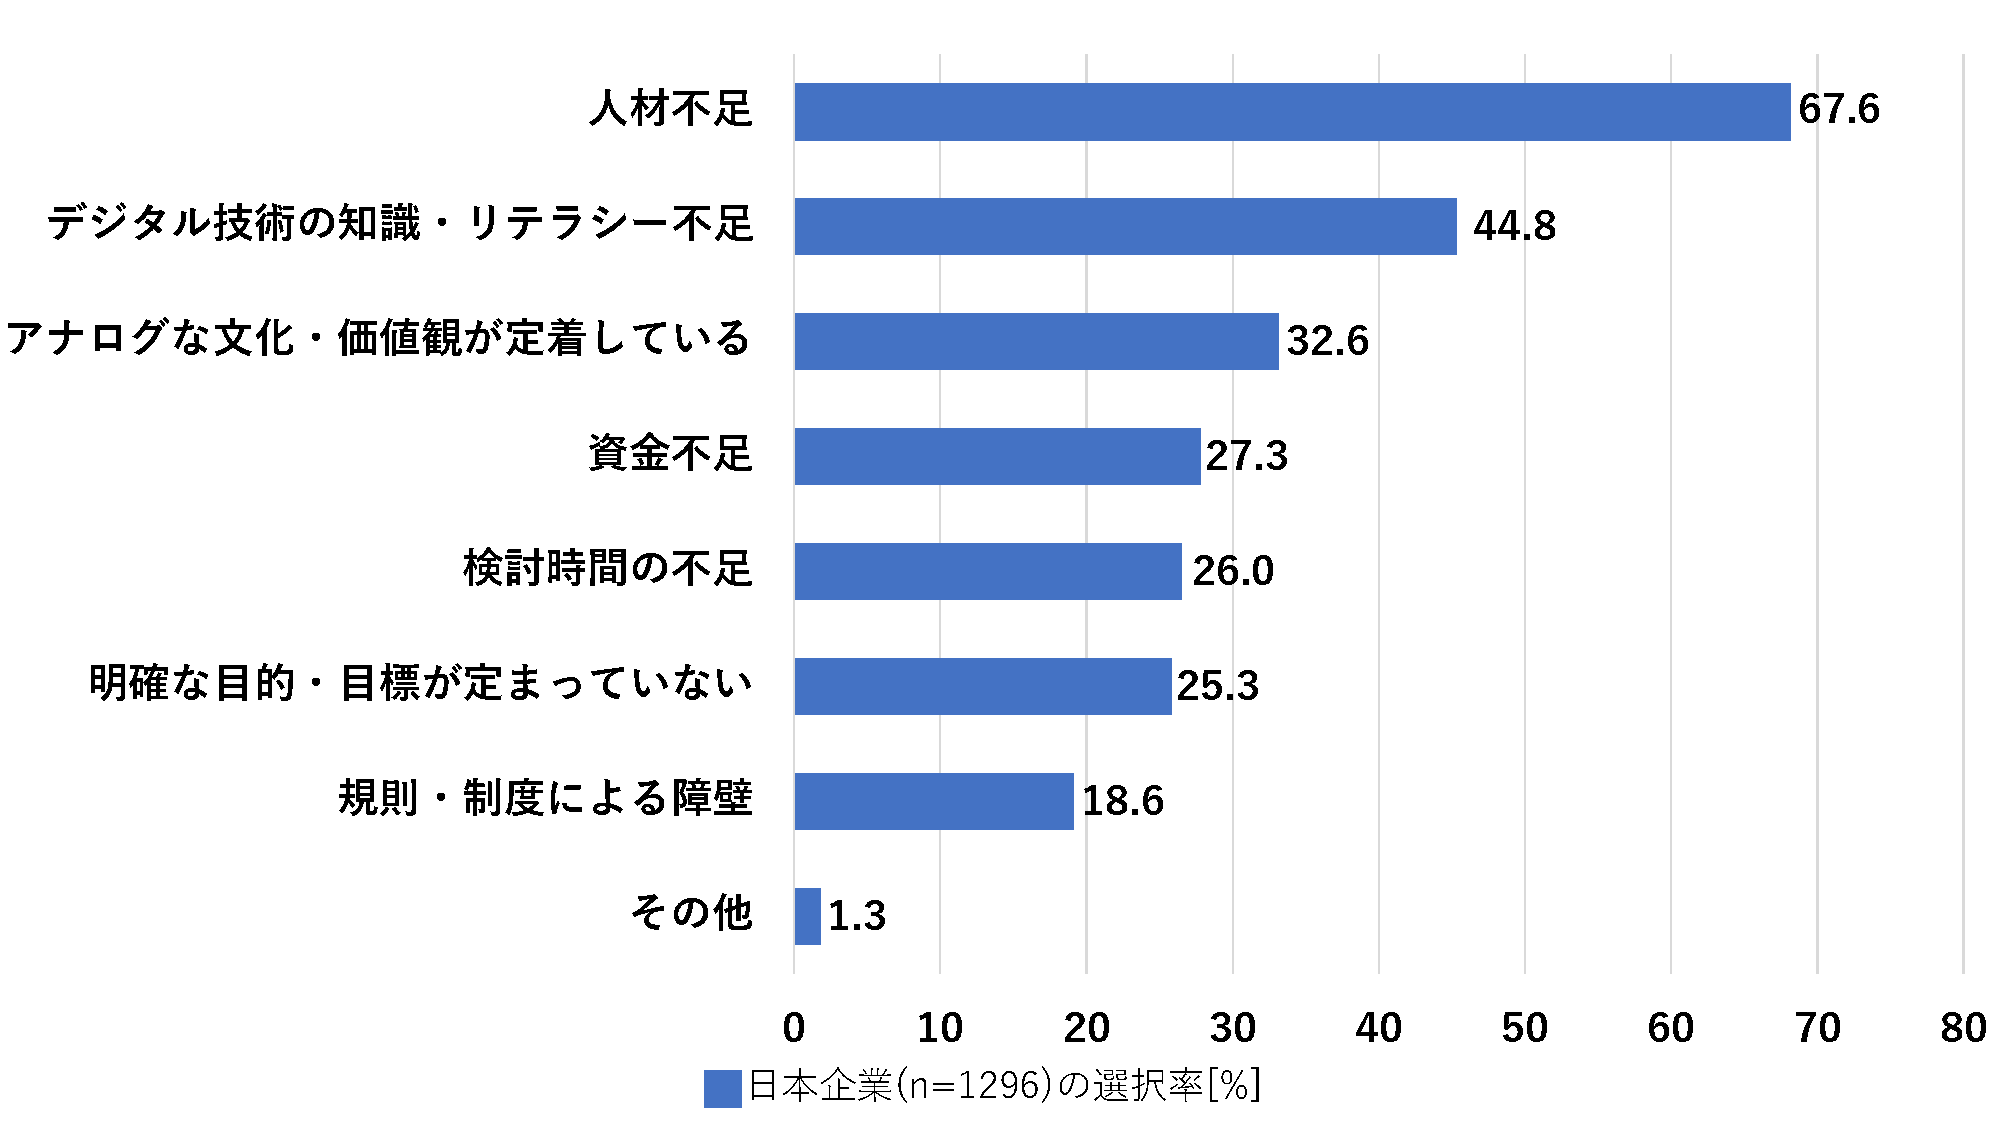
\includegraphics[clip,width=85mm,height=50mm]{figures/dx.pdf}
\caption[デジタル化を進める上での課題や障壁]{デジタル化を進める上での課題や障壁(複数選択)\linebreak}
\label{fig:dx}
\end{figure}

\clearpage
\section{情報教育について}
%本研究の目的と類似するものとして,電子版の教科書や教科書のQRコードを読み取り利用する,教科書付属のアニメーション教材が存在する.
%この教材の問題点として,短いアニメーションと文字のみで解説文との対応が無いこと,高等学校において電子版の教科書が普及していないことが挙げられる\cite{koukou_kyokasyo}.
\subsection{概要}
\subsection{情報教育におけるネットワークの学習内容}
\subsubsection{小学校プログラミング教育}
\subsubsection{中学校技術・家庭科(技術分野)内容「D 情報の技術」}
\subsubsection{高校「情報Ⅰ」}
\subsection{ネットワークの学習教材について}
\subsubsection{教科書付属のシミュレータ}
\subsubsection{「情報Ⅰ」動画教材}

\clearpage
\section{ネットワークの基礎知識}
\subsection{OSI}
\subsubsection{概要}
\subsubsection{OSI参照モデル}
\subsection{TCP/IP}
\subsubsection{概要}
\subsubsection{データリンク層}
\subsubsection{インターネット層}

\subsubsection{Ethernrtフレーム}
\begin{figure}[h]
\centering
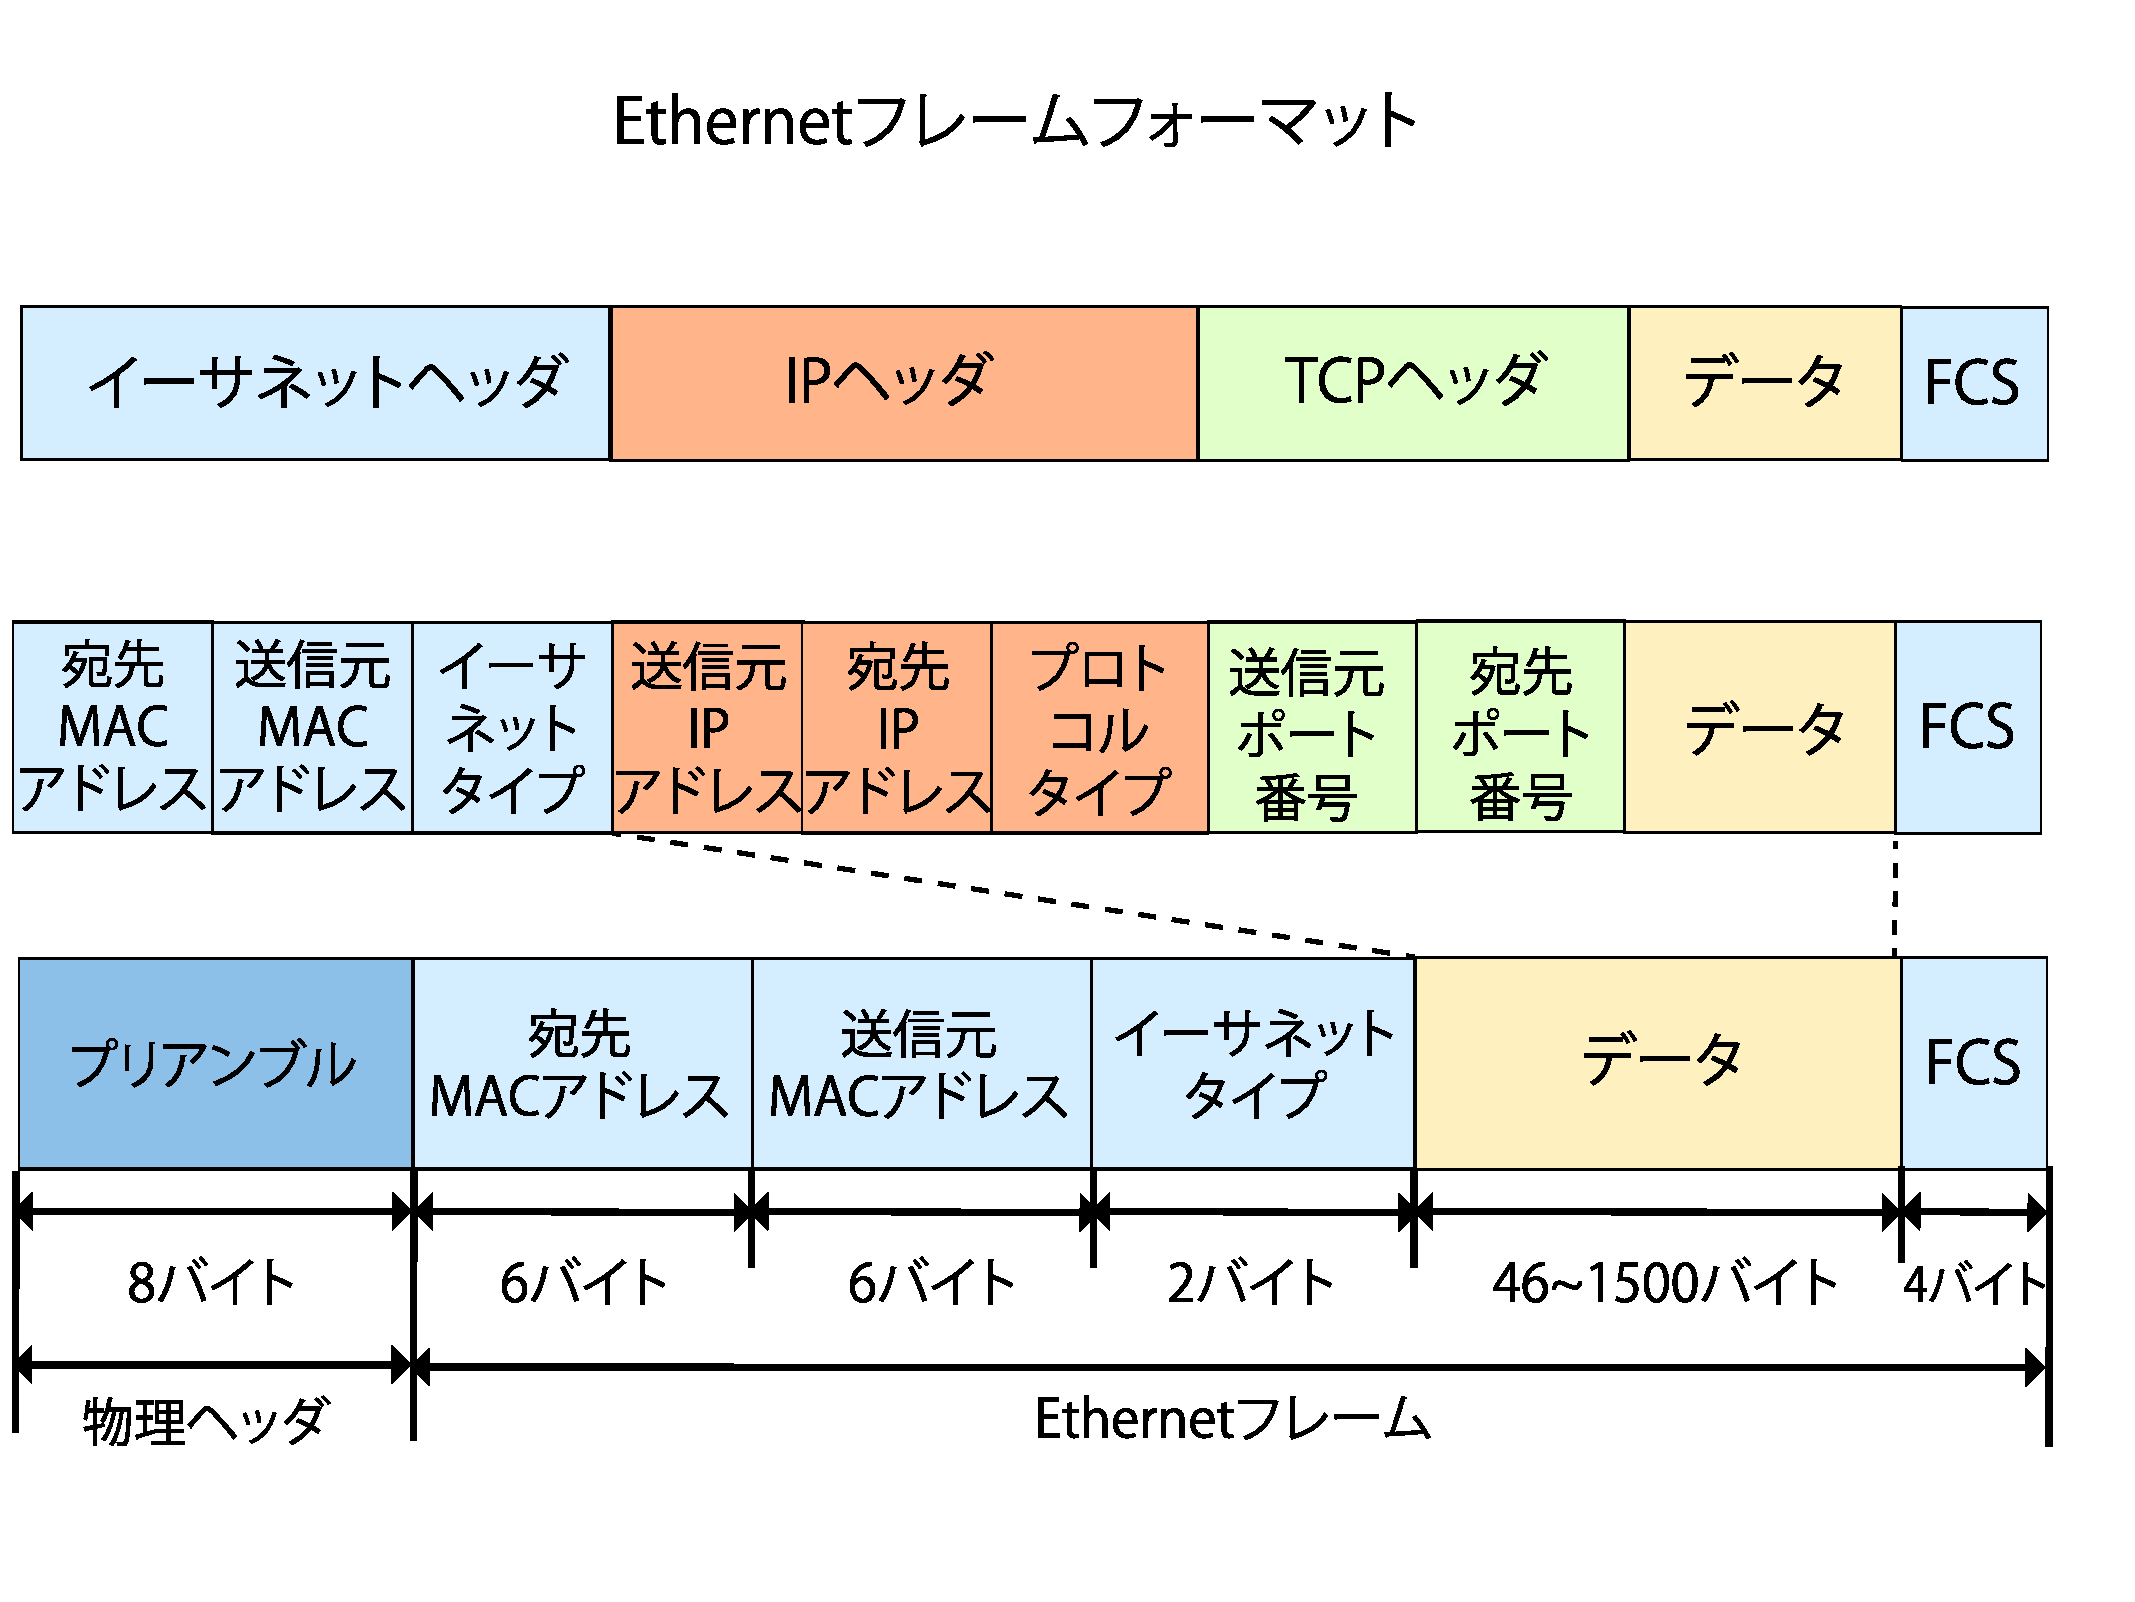
\includegraphics[clip,width=85mm,height=50mm]{figures/ethernet.pdf}
\caption[Ethernrtフレームの概略図]{Ethernrtフレームの概略図\linebreak}
\label{fig:ether}
\end{figure}

\subsubsection{IPアドレス}
\subsubsection{MACアドレス}

\clearpage
\section{開発する教材のコンセプト}
a
\subsection{学習目的}
\subsection{教材の利用環境}
\subsection{教材の学習内容}
\subsection{教材の画面設計}

\clearpage
\section{教材の画面構成}
\subsection{概要}

\begin{figure}[h]
\begin{center}
 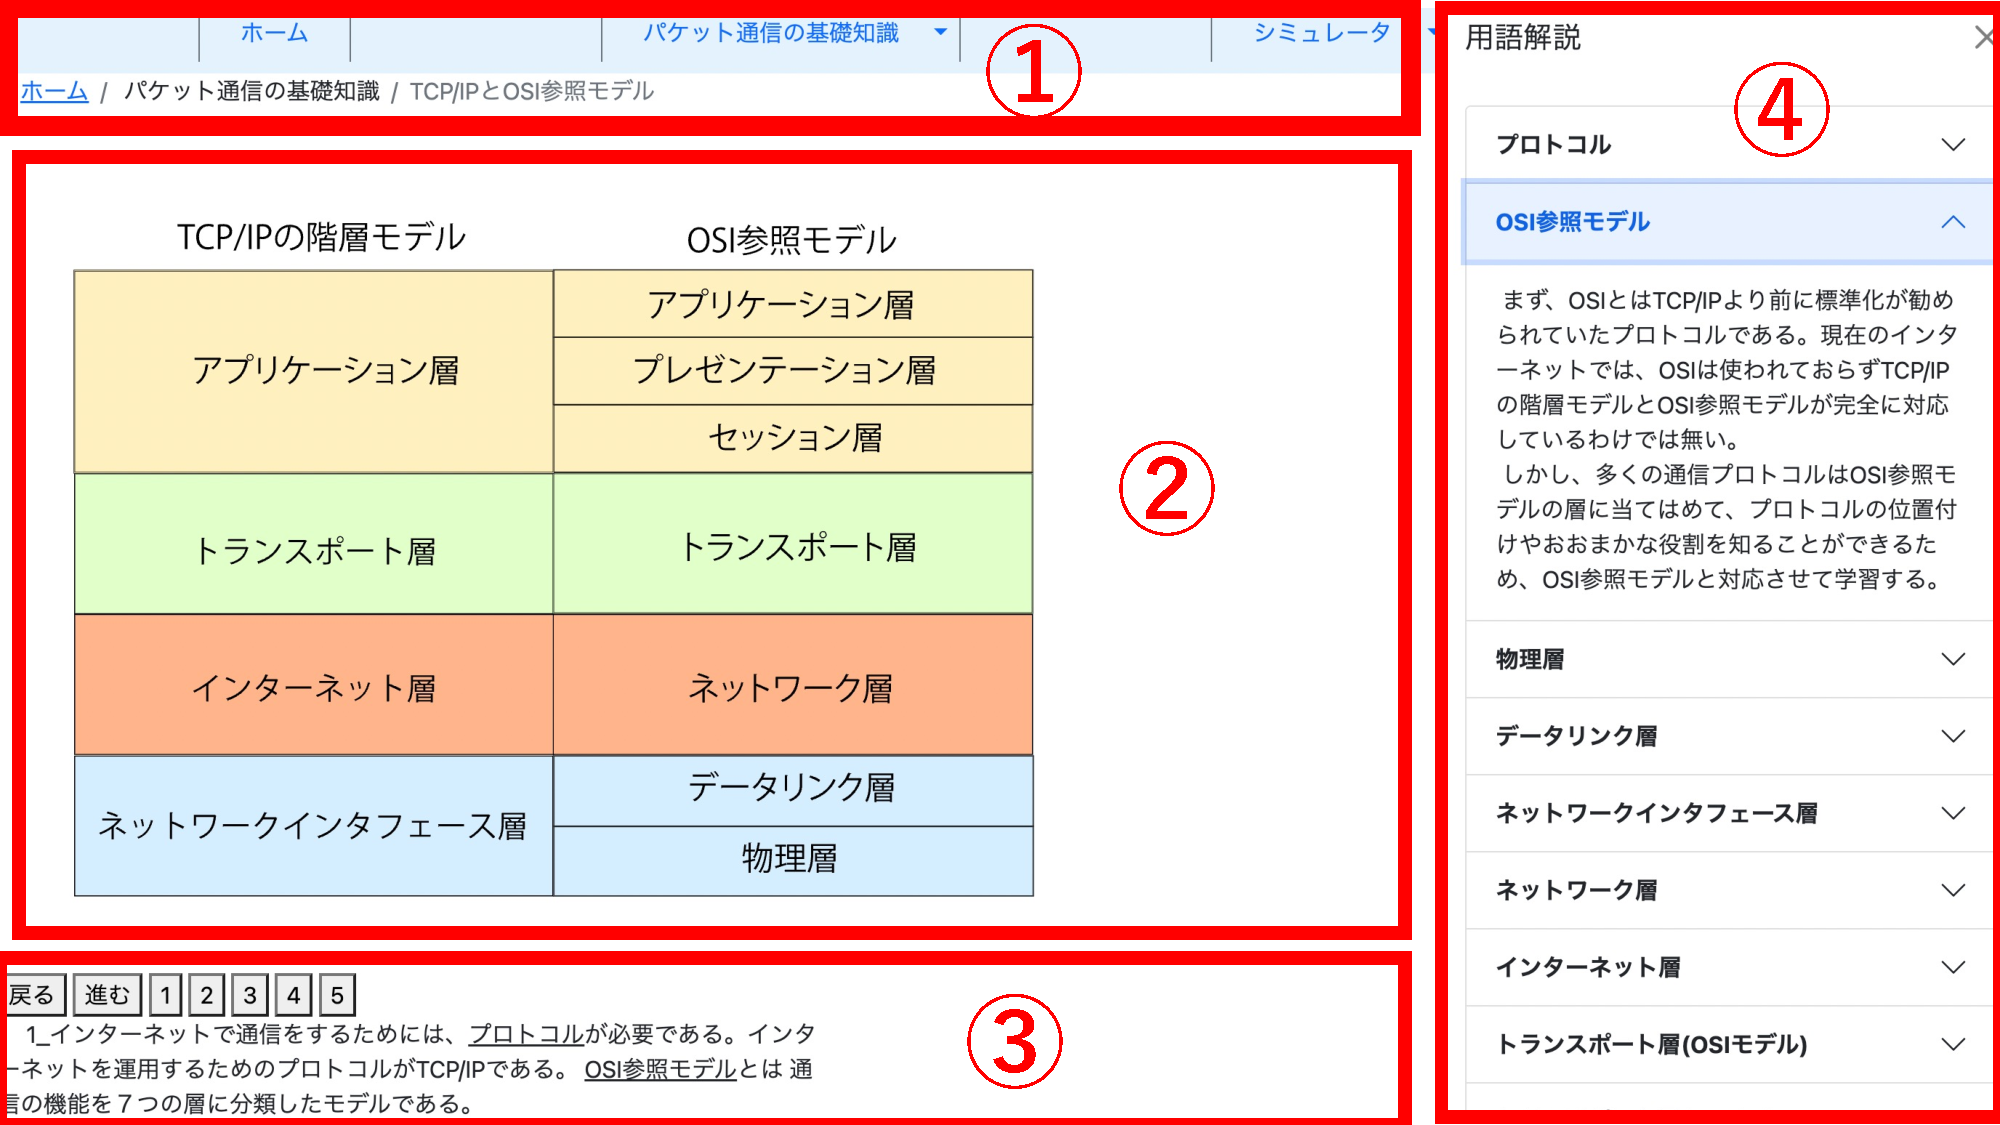
\includegraphics[clip,width=100mm,height=55mm]{figures/gamen.pdf}
\end{center}
 \caption{Web教材の学習画面}
 \label{fig:画面}
\end{figure}

\subsection{ナビゲーション部}
\subsection{メイン表示部}
\subsection{解説表示部}
\subsection{用語解説部}
\subsection{シミュレータ設定部}

\clearpage
\section{教材の実装}
a
\subsection{概要}
\subsection{開発に利用した言語}
\subsubsection{HTML}
\subsubsection{CSS}
\subsubsection{JavaScript}

\subsection{開発に利用したフレームワーク・ライブラリ}
\subsubsection{Bootstrap}
あ

\clearpage
\section{結言}
a
%本研究では,ネットワーク通信の基礎を学習する講義形式の授業を補助するWeb教材を開発した.今後このような,生徒や学生が自分で操作し学習できるWeb教材が普及し,講義形式の授業で学習内容を深く理解できるようになることを期待している.
\clearpage
\section{謝辞}
本研究の遂行及び本論文の作成にあたり,須田研究室の仲間に多くの手助けを頂きました,深く感謝の意を表します.そして,本論文の作成にあたり多大なる御指導及び御助言を頂きました,須田宇宙准教授に深く感謝の意を表します.
\clearpage

\begin{thebibliography}{99}

\bibitem{dx} 総務省: ``令和4年度版 情報通信白書'', p101,
\url{https://www.soumu.go.jp/johotsusintokei/whitepaper/ja/r04/pdf/n3800000.pdf}, 2022/8/16参照
\bibitem{koukou_sidou} 文部科学省: ``高等学校学習指導要領'', \url{https://www.mext.go.jp/a_menu/shotou/zyouhou/detail/mext_01831.html}, 2022/8/18参照
\bibitem{koukou_kyokasyo} 文部科学省: ``デジタル教科書に関する制度・現状について - 文部科学省'', \url{https://www.mext.go.jp/content/20200710-mxt_kyokasyo-000008653_03.pdf}, 2022/8/25参照
%https://ipsj.ixsq.nii.ac.jp/ej/?action=repository_uri&item_id=195372&file_id=1&file_no=1
\end{thebibliography}

\end{document}
